\subsection{Neural Network}

A number of these sigmoid neurons (or neurons with other activation functions) can be strung together to make a neural network \cite{Budinger_2014}.
Each neural network has 3 main parts.

\begin{figure}[H]
  \centering
  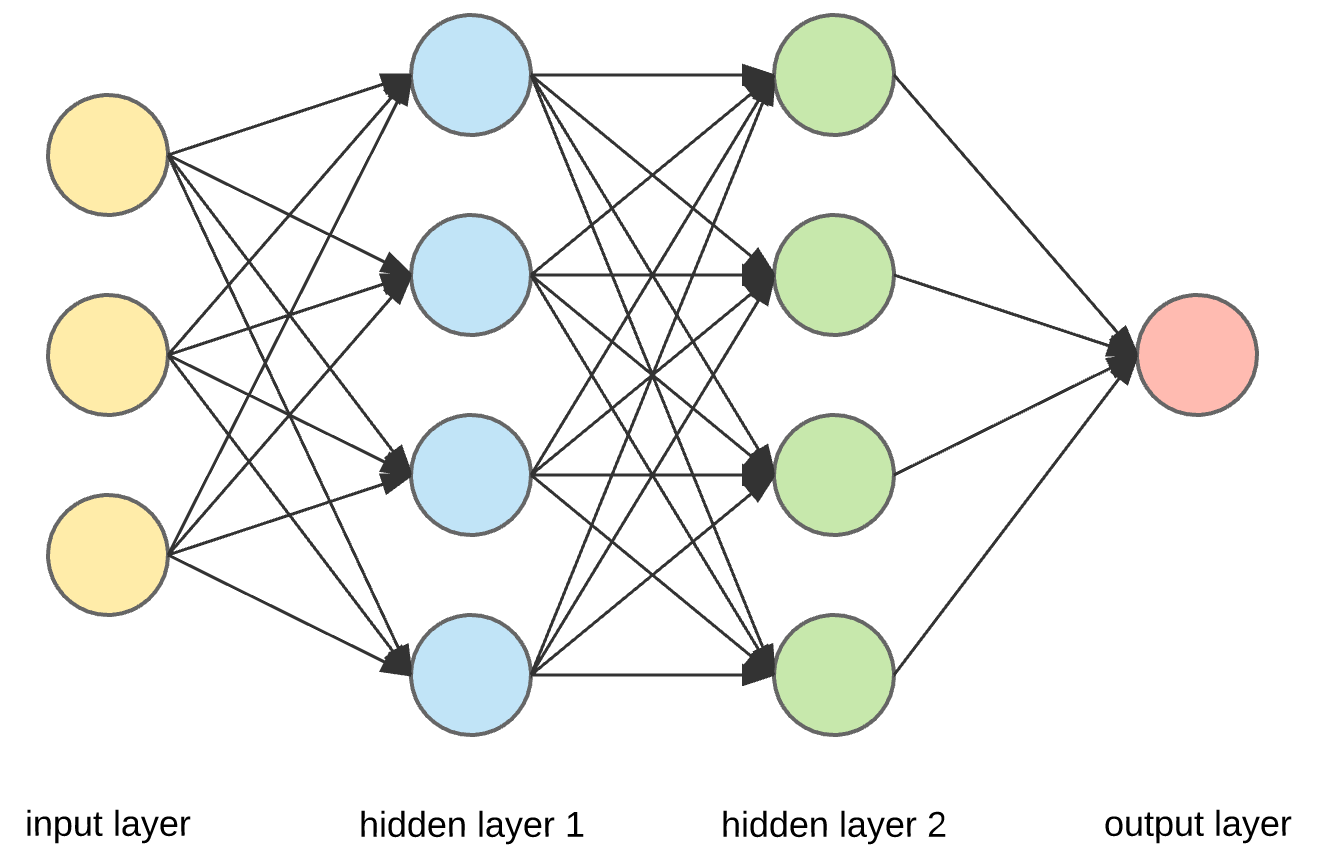
\includegraphics[width=120mm]{figures/neuralNet1.png}
  \caption{Parts of a Neural Net \cite{Lelli_2019}}
  \label{neuralNet2}
\end{figure}

First, we have an input layer.
This is all the inputs that go into a neural network and is usually represented as a vector.
Each input adds one to the dimension of the input vector.
Even something like a 2d picture can have its rows stitched together to make one long vector of inputs \cite{Bishop_2016}.

The middle bits are called the hidden layer, not for any profound reason, but just to distinguish them from the input and output layers.
You can have as many hidden middle layers as you want in the network.
The trade off is usually one of efficiency and accuracy.
The more hidden layers you have, the more accurate the output will be but at the cost of requiring more time to train because there are more weights to get right.
After a point, adding more layers does not improve accuracy in meaningful way while still taking longer to train \cite{Antoniadis_2024}.
This makes creating a good neural net less of a hard science and more of an art form.

Finally, we have the output layer.
This layer usually has one neuron for each thing the classifier can bin the input into \cite{Bishop_2016}.
In the dog and cat case, we would have $2$ output neurons, one that signifies dog and the other cat.
However, the neurons won't directly tell us whether the picture contains a dog or a cat but rather give us two values.
One of these values indicates how likely it is for this picture to contain a cat and the other represents the likelihood that the picture contains a dog.
After that, it is still up to us to decide on cutoff values to determine whether we will say the picture contains a cat, a dog, both or neither.
